% MEI impedance meter, divider version as simulated in LTspice/ngspice (Pico replaced by sources).
% Compile: pdflatex mei_circuit_ltspice.tex
\documentclass[border=12pt]{standalone}
\usepackage[american]{circuitikz}
\usepackage{amsmath}
\usetikzlibrary{calc}
\ctikzset{bipoles/length=1.5cm}
\tikzset{every picture/.append style={font=\small}}

% voltage follower: name, x of (+) input, y of (+) input, label, feedback drop (cm)
\newcommand{\follower}[5]{%
  \node[op amp, noinv input up, anchor=+] (#1) at (#2,#3) {};
  \node[font=\scriptsize, align=center] at ([yshift=0.7cm]#1.up) {#4};
  \coordinate (#1o) at ($(#1.out)+(0.8,0)$);
  \coordinate (#1l) at ($(#1.-)+(-0.6,-#5)$);
  \draw (#1.out) -- (#1o) -- (#1o |- #1l) -- (#1l) -- (#1l |- #1.-) -- (#1.-);
  \fill (#1o) circle (1.4pt);
}

\begin{document}
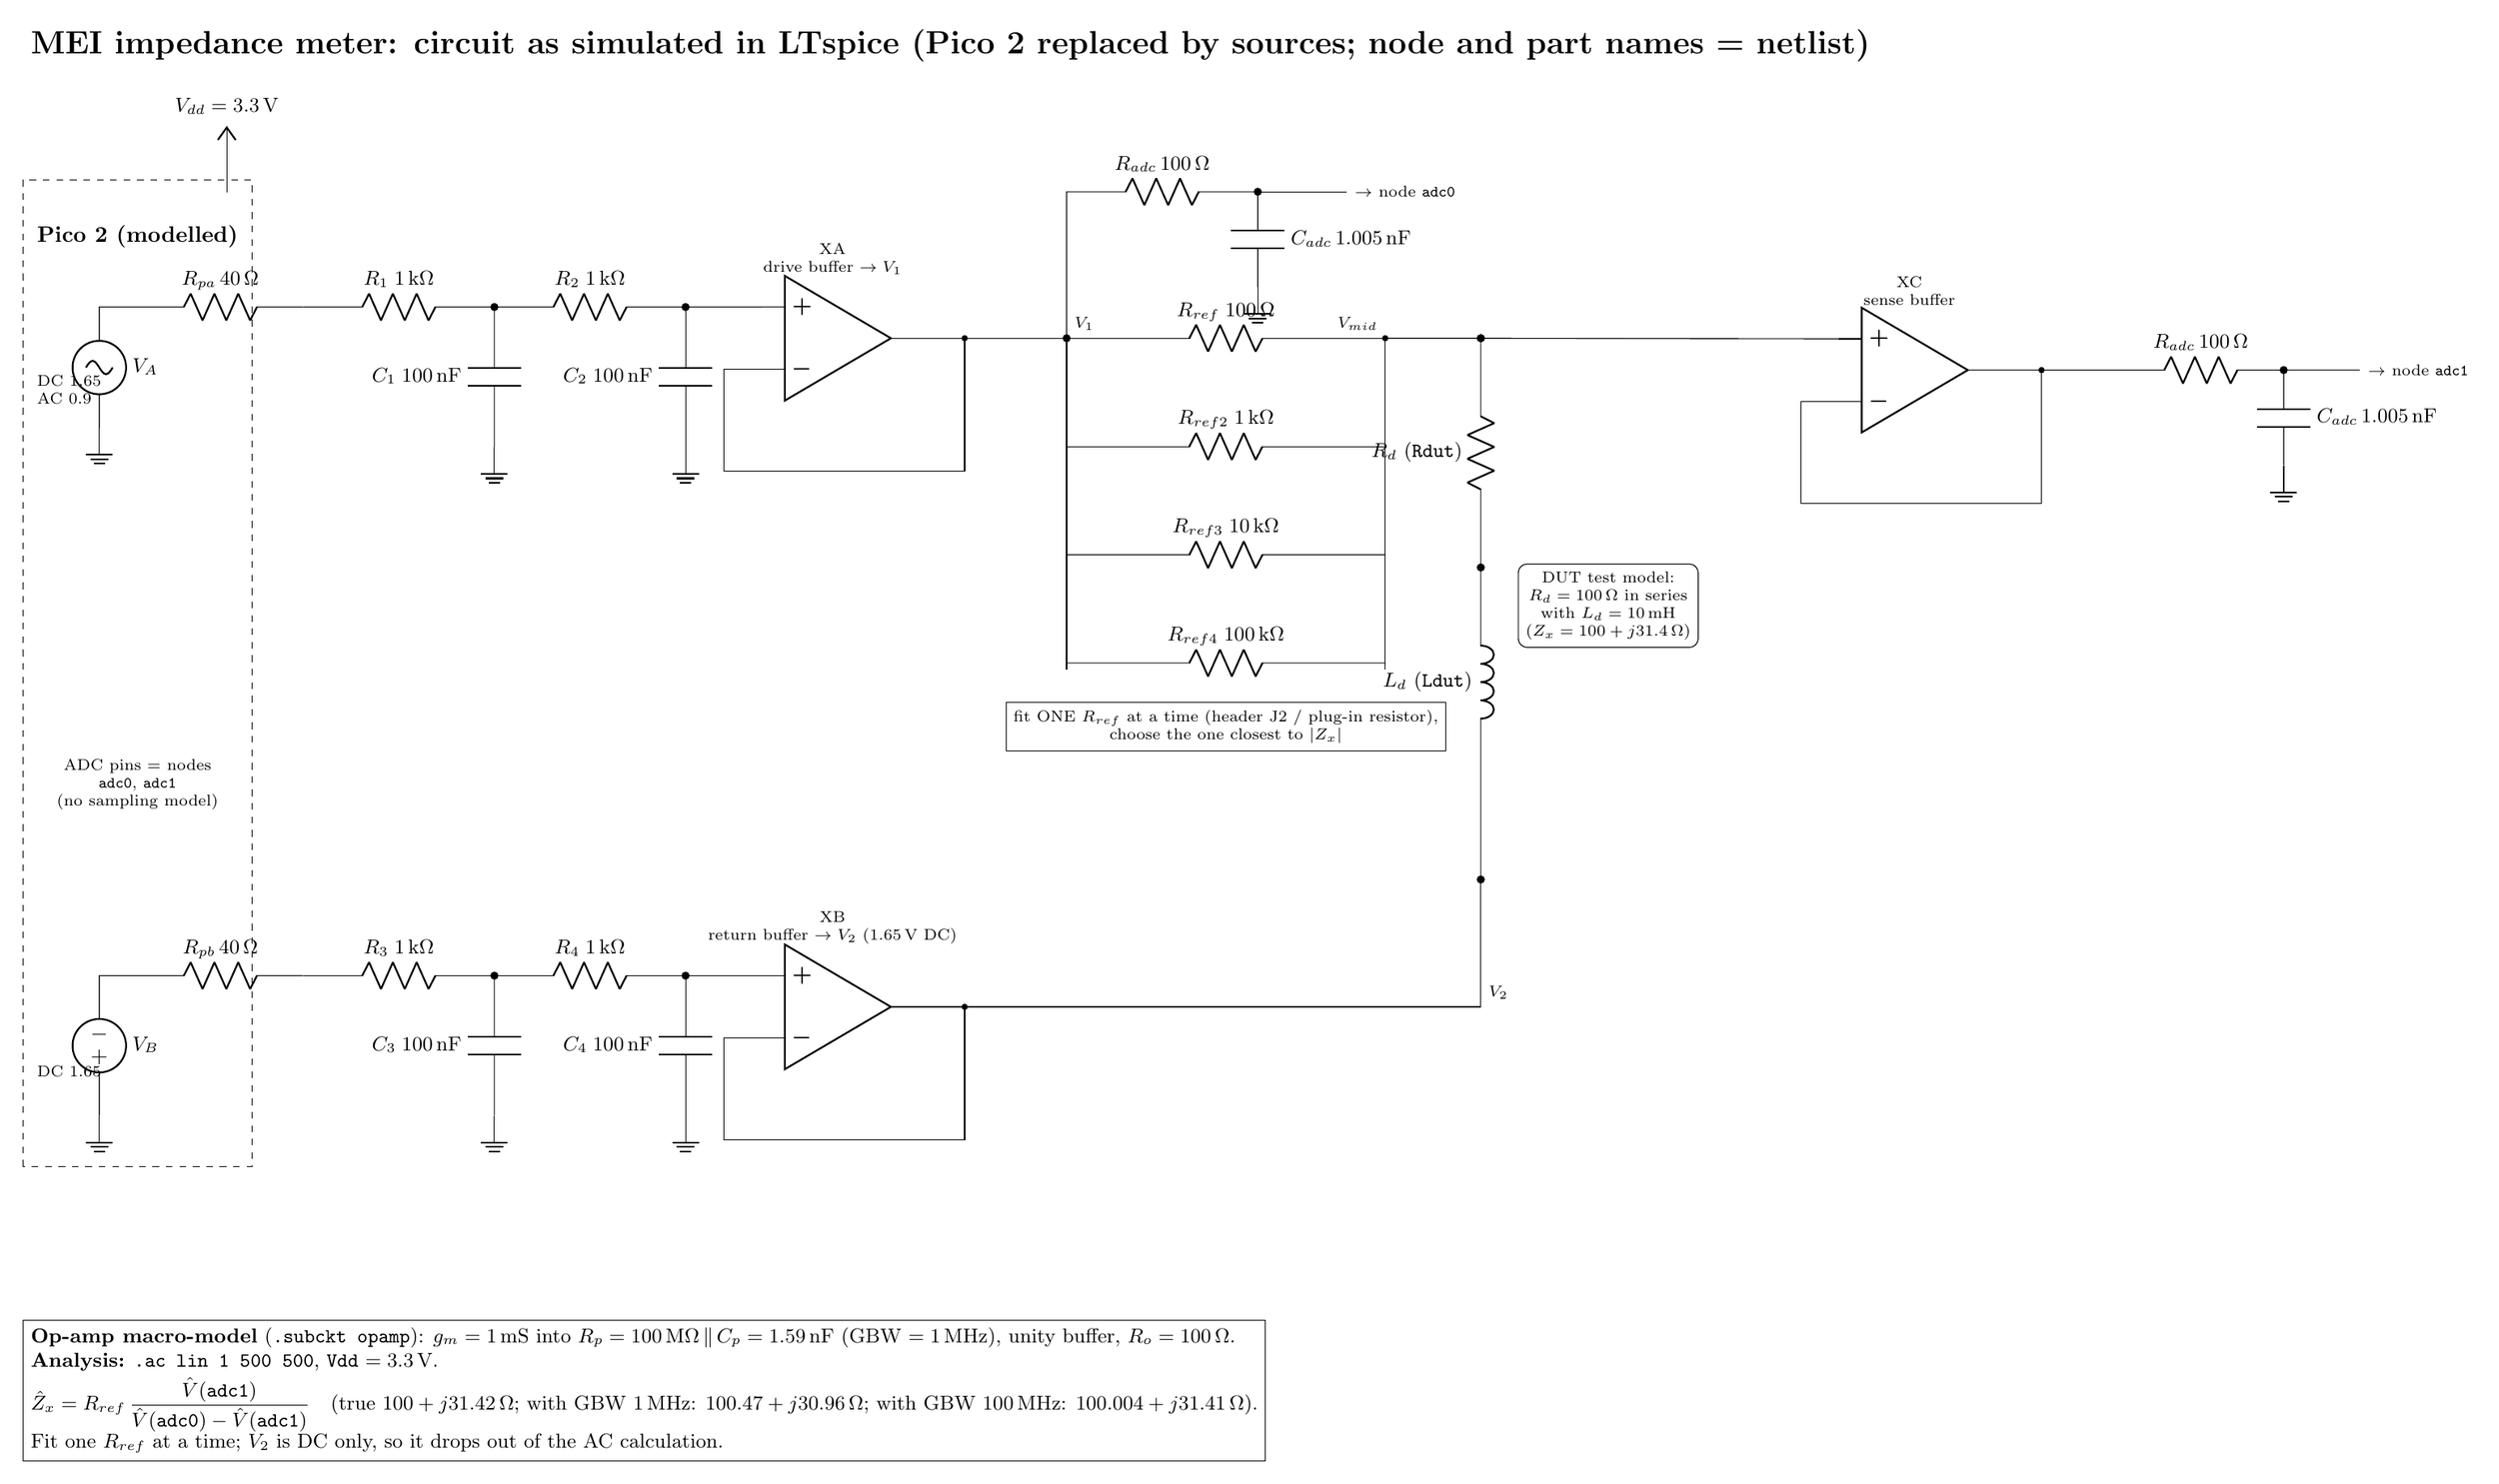
\begin{tikzpicture}
\node[font=\Large\bfseries, anchor=west] at (0,8.6)
  {MEI impedance meter: circuit as simulated in LTspice (Pico 2 replaced by sources; node and part names = netlist)};

% ---------------- Pico 2 replaced by sources ----------------
\draw[dashed] (0,-9) rectangle (3.6,6.5);
\node[font=\bfseries,align=center] at (1.8,5.6) {Pico 2 (modelled)};
% VA: 1.65 V DC + 0.9 V AC (500 Hz), then 40 ohm pin resistance
\draw (1.2,2.6) node[ground]{} to[sV, l_=$V_A$] (1.2,4.5) -- (1.8,4.5) to[R, l=$R_{pa}$\,40\,$\Omega$] (4.4,4.5);
\node[font=\scriptsize,align=left,anchor=west] at (0.1,3.2) {DC 1.65\\ AC 0.9};
% VB: 1.65 V DC, 40 ohm
\draw (1.2,-8.2) node[ground]{} to[V, l_=$V_B$] (1.2,-6) -- (1.8,-6) to[R, l=$R_{pb}$\,40\,$\Omega$] (4.4,-6);
\node[font=\scriptsize,align=left,anchor=west] at (0.1,-7.5) {DC 1.65};
\node[font=\scriptsize,align=center] at (1.8,-3) {ADC pins = nodes\\ \texttt{adc0}, \texttt{adc1}\\ (no sampling model)};
\draw (3.2,6.3) -- (3.2,6.9) node[vcc]{$V_{dd}=3.3$\,V};

% ---------------- Channel A: PWM A -> RC -> RC -> follower U1A -> V1 ----------------
\draw (4.4,4.5) to[R, l=$R_1\;1\,\mathrm{k\Omega}$] (7.4,4.5) node[circ]{} coordinate(a1)
      to[R, l=$R_2\;1\,\mathrm{k\Omega}$] (10.4,4.5) node[circ]{} coordinate(a2) -- (11.6,4.5);
\draw (a1) to[C, l_=$C_1\;100\,\mathrm{nF}$] ++(0,-2.2) node[ground]{};
\draw (a2) to[C, l_=$C_2\;100\,\mathrm{nF}$] ++(0,-2.2) node[ground]{};
\follower{A1}{11.6}{4.5}{XA\\ drive buffer $\to V_1$}{1.6}

% ---------------- Channel B: PWM B (50 % duty) -> RC -> RC -> follower U1B -> V2 (mid-rail) ----
\draw (4.4,-6) to[R, l=$R_3\;1\,\mathrm{k\Omega}$] (7.4,-6) node[circ]{} coordinate(b1)
      to[R, l=$R_4\;1\,\mathrm{k\Omega}$] (10.4,-6) node[circ]{} coordinate(b2) -- (11.6,-6);
\draw (b1) to[C, l_=$C_3\;100\,\mathrm{nF}$] ++(0,-2.2) node[ground]{};
\draw (b2) to[C, l_=$C_4\;100\,\mathrm{nF}$] ++(0,-2.2) node[ground]{};
\follower{A2}{11.6}{-6}{XB\\ return buffer $\to V_2$ (1.65\,V DC)}{1.6}

% ---------------- V1 node and ADC0 tap ----------------
\draw (A1o) -- ++(1.6,0) coordinate(V1) node[circ]{};
\node[above right,font=\scriptsize] at (V1) {$V_1$};
\draw (V1) -- ++(0,2.3) to[R, l=$R_{adc}\,100\,\Omega$] ++(3,0) node[circ]{} coordinate(n0)
      to[C, l=$C_{adc}\,1.005\,\mathrm{nF}$] ++(0,-1.5) node[ground]{};
\draw (n0) -- ++(1.4,0) node[right,font=\scriptsize]{$\to$ node \texttt{adc0}};

% ---------------- Reference resistor ranges (fit ONE) ----------------
\coordinate (Vm) at ($(V1)+(5,0)$);
\draw (V1) -- ++(0,-5.2);
\draw (Vm) -- ++(0,-5.2);
\draw (V1) to[R, l=$R_{ref}\;100\,\Omega$] (Vm);
\foreach \k/\val in {1/{1\,\mathrm{k\Omega}},2/{10\,\mathrm{k\Omega}},3/{100\,\mathrm{k\Omega}}}{
  \draw ($(V1)+(0,-1.7*\k)$) to[R, l=$R_{ref\the\numexpr\k+1\relax}\;\val$] ($(Vm)+(0,-1.7*\k)$);
}
\node[font=\scriptsize, align=center, fill=white, draw] at ($(V1)!0.5!(Vm)+(0,-6.1)$)
  {fit ONE $R_{ref}$ at a time (header J2 / plug-in resistor),\\ choose the one closest to $|Z_x|$};

% ---------------- Vmid node, DUT and U1C ----------------
\fill (Vm) circle (1.4pt);
\node[above left,font=\scriptsize] at (Vm) {$V_{mid}$};
\draw (Vm) -- ++(1.5,0) node[circ]{} coordinate(Dt) -- (28.5,4.0);
\follower{A3}{28.5}{4.0}{XC\\ sense buffer}{1.6}
\draw (A3o) -- ++(0.0,0);
\draw (A3o) -- ++(1.2,0) to[R, l=$R_{adc}\,100\,\Omega$] ++(2.6,0) node[circ]{} coordinate(n1)
      to[C, l=$C_{adc}\,1.005\,\mathrm{nF}$] ++(0,-1.5) node[ground]{};
\draw (n1) -- ++(1.2,0) node[right,font=\scriptsize]{$\to$ node \texttt{adc1}};
% DUT
\draw (Dt) to[R, l_=$R_d$ (\texttt{Rdut})] ++(0,-3.6) node[circ]{} to[L, l_=$L_d$ (\texttt{Ldut})] ++(0,-3.6) -- ++(0,-1.3) coordinate(Db);
\node[draw, rounded corners, font=\scriptsize, align=center, fill=white] at ($(Dt)+(2.0,-4.2)$)
  {DUT test model:\\ $R_d=100\,\Omega$ in series\\ with $L_d=10$\,mH\\ ($Z_x=100+j31.4\,\Omega$)};
\draw (A2o) -- ++(0,0);
\draw (A2o) -- (A2o -| Db) -- (Db) node[circ]{};
\node[above right,font=\scriptsize] at (A2o -| Db) {$V_2$};
\node[circ] at (Dt) {};

% ---------------- Equations ----------------
\node[draw, align=left, font=\small, anchor=north west, fill=white] at (0,-11.4)
{\textbf{Op-amp macro-model} (\texttt{.subckt opamp}): $g_m=1$\,mS into $R_p=100$\,M$\Omega\,\|\,C_p=1.59$\,nF (GBW $=1$\,MHz), unity buffer, $R_o=100\,\Omega$.\\
\textbf{Analysis:} \texttt{.ac lin 1 500 500}, \texttt{Vdd} $=3.3$\,V.\\[2pt]
$\displaystyle \hat Z_x=R_{ref}\,\frac{\hat V(\mathtt{adc1})}{\hat V(\mathtt{adc0})-\hat V(\mathtt{adc1})}$\quad
 (true $100+j31.42\,\Omega$; with GBW 1\,MHz: $100.47+j30.96\,\Omega$; with GBW 100\,MHz: $100.004+j31.41\,\Omega$).\\
Fit one $R_{ref}$ at a time; $V_2$ is DC only, so it drops out of the AC calculation.};
\end{tikzpicture}
\end{document}
